\lecture{异常处理}{lec:chap10}
\section[概述]{异常处理概述}\label{sec:chap10-sec01}
%%%%%%%%%%%%%%%%%%%%%%%%%%%%%%%%%%%%%%%%
\begin{frame}[t, fragile]{异常处理概述}%
  \begin{itemize}
  \item 错误:语法错误,逻辑错误和运行错误。
    \begin{itemize}
      \scriptsize
    \item 语法错误:程序中不符合语法规则之处,可由编译器检测出来,如非
      法标识符、不完整的控制结构等。
    \item 逻辑错误:程序逻辑有问题,导致得不到预期结果,可通过调试和测
      试解决,如条件错误等。
    \item \alert{异常(exception)}:程序运行过程中可以检测到的非正常情况,如除数为0、数组下标越界、内存分配失败、运算溢出、文件打开失败、函数实参无效等。
    \end{itemize}
  \end{itemize}  
\end{frame}

\begin{frame}[t, fragile]{异常处理概述}%
  \begin{itemize}
  \item 常见的错误处理方法
    \begin{itemize}      
    \item 使用断言
      \begin{itemize}
      \item 断言主要用于开发和维护阶段,用于处理不该发生的非法情况,如
        指针非空检测、参数合法性验证等。      
      \end{itemize}
    \item \cppinline{<cassert>}中提供一个参数宏\cppinline{<assert>}:
  \begin{itemize}
  \item 函数原型: \cppinline{void assert (int expression);}
  \item assert仅用于程序的调试版。如果表达式的值为0,则输出出错信息,并
    调用abort()结束程序。
  \end{itemize}  
  \end{itemize}  
\end{itemize}
\end{frame}

\begin{frame}[t, fragile]{异常处理概述}%
  \begin{itemize}
  \item 常见的错误处理方法
    \begin{itemize}
    \item 异常处理
      \begin{itemize}
      \item 一般的程序错误尽量避免使用异常
      \item 避免在构造和析构函数中抛出异常
      \item 在异常对象中包含必要的异常信息
      \end{itemize}
    \item 结束程序:调用abort或exit函数结束应用程序
    \item 局部处理
    \item 忽略错误
    \item setjump/longjump
    \end{itemize}
  \end{itemize}
\end{frame}

\begin{frame}[t, fragile]{异常处理概述}%
  \begin{itemize}
  \item \alert{异常处理机制}是程序设计语言提供的一种用于管理程序运行异
    常的结构化方法
    \begin{itemize}
      \item 允许将正常处理代码与异常处理代码明显分开,以提高程序的可读
        性和可维护性。
      \item 允许异常检测与异常处理相分离,使得独立开发的两部分程序之间进行异常通信,允许用户选择处理异常的方式,以提高程序的健壮性。
    \end{itemize}    
  \end{itemize}
\end{frame}

%%%%%%%%%%%%%%%%%%%%%%%%%%%%%%%%%%%%%%%%

\section[机制]{异常处理机制}\label{sec:chap10-sec02}
%%%%%%%%%%%%%%%%%%%%%%%%%%%%%%%%%%%%%%%%
\begin{frame}[t, fragile]{try-catch语句}%
  \begin{itemize}
  \item try-catch
  \end{itemize}
  \begin{center}
    \begin{tikzpicture}[font=\tiny, show background grid]
      \tikzset{coord/.style={coordinate}}

      \umlnote[scale=0.9, text width=0.3\textwidth] (code1) at (0, 0)
      {
        \begin{cpptt}
          try
          {
            // 语句
          }
        \end{cpptt}
      };

      \umlnote[scale=0.9, text width=0.5\textwidth] (txtnode1) at (4.5, 0)
      {
        \begin{cpptt}
          |异常抛出区:将可能抛出异常的代码置于try块内。|
          |当检测到本身无法处理的异常时,|
          |采用throw语句抛出异常。|
        \end{cpptt}
      };

      \umlnote[scale=0.9, text width=0.3\textwidth] (code2) at (0, -2)
      {
        \begin{cppttnobg}
          catch( |类型名| [|形参名|])
          {
            // 语句
          }
          catch( |类型名| [|形参名|])
          {
            // 语句
          }
          |...|
          catch(|…|)
          {
            // 语句
          }
        \end{cppttnobg}
      };

      \umlnote[scale=0.9, text width=0.5\textwidth] (txtnode2) at (4.5, -2)
      {
        \begin{cppttnobg}
          |异常处理区:|
          |try块后面紧跟一个或多个catch块,|
          |用于捕获并处理异常。|
        \end{cppttnobg}
      };
    \end{tikzpicture}
  \end{center}
\end{frame}

\begin{frame}[t, fragile]{try块(try block)}%
  \begin{itemize}
  \item 将可能抛出异常的代码放在try块内
    \begin{itemize}
    \item 语法形式:\\
      \begin{cpptt}
        try
        {
          //可能产生异常的代码
        }
      \end{cpptt}
    \item try块通常置于函数体内,也可以是\alert{函数try块}
    \item try块主要用于检测异常,采用throw语句抛出异常
    \item try块后紧跟一个或多个catch子句
    \end{itemize}
  \end{itemize}
\end{frame}


\begin{frame}[t, fragile]{throw语句}%
  \begin{itemize}
  \item throw语句用于抛出某种类型的异常
    \begin{itemize}
    \item 语法形式:\\
      \begin{cpptt}
        throw |表达式|;
      \end{cpptt}
    \item 表达式可以是单个对象,其类型指明了\alert{异常类型},其值用于
      创建一个\alert{异常对象}(存储在专用的异常栈而非函数栈)。如:
      \cppinline{throw 'x';  throw string();}
    \item 空的throw语句表示\alert{重新抛出}原先的异常对象,一般置于
      catch子句中,如:\cppinline{throw;}
    \item 抛出异常后,程序跳出当前的try块,并根据异常类型搜索匹配的
      catch子句来捕获并处理异常
    \end{itemize}
  \end{itemize}
\end{frame}

\begin{frame}[t, fragile]{catch子句}%
  \begin{itemize}
  \item catch子句负责捕获并处理try块中抛出的异常
    \begin{itemize}
    \item 语法形式:\\
      \begin{cpptt}
        catch(|异常声明|)
        {
          // 异常处理代码
        }
      \end{cpptt}
    \item 异常声明可以是一个类型名、一个对象声明或$\cdots$
      \begin{itemize}
      \item 类型名表示该catch子句能够捕获的异常类型
      \item 对象名称用于在异常处理代码中引用异常对象
      \item $\cdots$表示可以捕获所有异常
      \end{itemize}
    \end{itemize}
  \end{itemize}
\end{frame}

\begin{frame}[t, fragile]{catch子句}%
  \begin{itemize}
  \item 当抛出的异常对象与catch子句的异常类型相同,或者是其派生类型时,则由该catch子句捕获并处理异常,异常对象通过catch形参传给catch子句。
    \begin{itemize}
    \item 如果希望在catch子句中访问异常对象,则应该声明catch形参,否则
      指定异常类型名即可。
    \item 如果希望在catch子句中修改异常对象,则应该catch形参声明为\alert{引用
      或指针},否则catch子句不会修改原先的异常对象,修改的只是原异常对
      象的副本。
    \item 如果catch子句不能完全处理异常,则可以用空的throw语句\alert{重新抛出
      异常},由其调用链的上层处理。
    \end{itemize}
  \end{itemize}
\end{frame}

\begin{frame}[t, fragile]{catch子句}%
  \begin{itemize}
  \item 异常类型匹配是按照catch子句的先后顺序进行的,一旦匹配成功,则转入对应的catch子句,不会再与其后的catch子句进行匹配。
    \begin{itemize}
    \item catch(…)子句应放在最后;
    \item 异常派生类的catch子句应置于对应异常基类的catch子句之前。
    \end{itemize}
  \end{itemize}
\end{frame}

\begin{frame}[t, fragile]{异常处理流程}%
  \begin{itemize}
  \item 如果try块没有抛出异常,则跳过与当前try块关联的catch子句,继续
    执行其他代码。
  \item 如果异常抛出语句没有包含在try块中,则调用terminate函数结束程序。
  \item 如果try块的代码抛出异常,则跳过try块中抛出点之后的代码,逐层向
    上搜索匹配的catch子句来处理异常,搜索过程如下:
    \begin{itemize}
    \item 先在与当前try块关联的catch子句中搜索,如果没有找到,则退出当
      前层次,继续在其上层try块关联的catch子句中搜索。如果找到,则由匹
      配的catch子句处理异常,处理完毕后跳过当前层次的其余catch子句,继
      续其他代码;如果搜索到主函数仍未捕获异常,则调用terminate函数结束
      程序。
    \end{itemize}
  \end{itemize}
\end{frame}

%%%%%%%%%%%%%%%%%%%%%%%%%%%%%%%%%%%%%%%%

\section[规范]{异常规范}\label{sec:chap10-sec03}
%%%%%%%%%%%%%%%%%%%%%%%%%%%%%%%%%%%%%%%%
\begin{frame}[t, fragile]{catch}%
  \begin{itemize}
  \item C++的异常处理代码是catch子句。当一个异常被try块中的语句抛出时,
    系统在try块后的catch子句列表中查找能够处理该异常的catch子句。    
  \end{itemize}  
\end{frame}
%%%%%%%%%%%%%%%%%%%%%%%%%%%%%%%%%%%%%%%%

\section[异常类]{标准库的异常类}\label{sec:chap10-sec04}
%%%%%%%%%%%%%%%%%%%%%%%%%%%%%%%%%%%%%%%%

%%%%%%%%%%%%%%%%%%%%%%%%%%%%%%%%%%%%%%%%
% 附件页
\section[附件下载]{本讲示例代码及附件下载} 
\begin{frame}{附件}{本讲附件}
  % 此处的[ucfilespec=...]必须指定为pdf否则Windows下无法下载
  %\vspace{-4ex}
  \textattachfile[ucfilespec=ex-src10.pdf]{ex-src10.zip}{附件:右键单击该
    链接,选择\qtmark{\alert{保存附件}}下载,\alert{将后缀名改为\qtmark{.zip}解压}
      \footnote[frame]{请\alert{退出全屏模式}后点击该链接。}
      \footnote[frame]{以Adobe Acrobat Reader为例。}
      。}%\\

  \vspace{-1ex}
  \begin{center}
    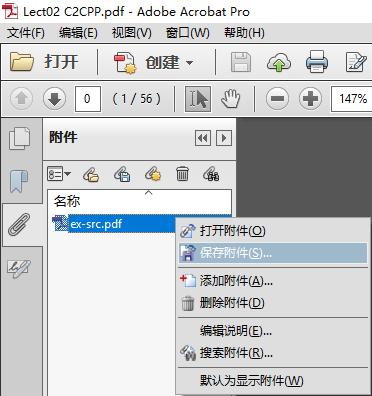
\includegraphics[height=0.35\textheight]{pdfattatchdownload01}\quad
    %或 \quad%
    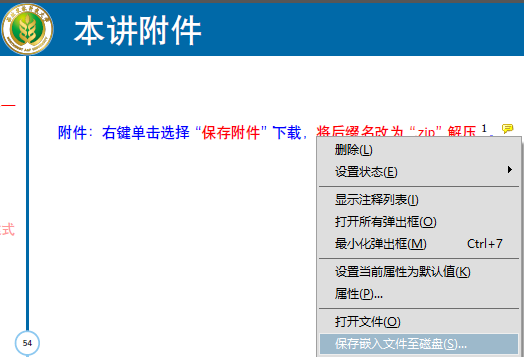
\includegraphics[height=0.35\textheight]{pdfattatchdownload02}\\[2ex]%
    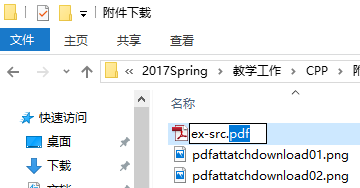
\includegraphics[height=0.255\textheight]{pdfattatchdownload03}\quad
    %$\Rightarrow$ \quad%
    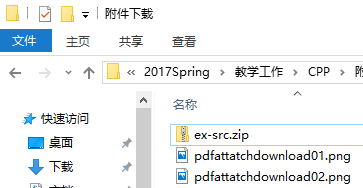
\includegraphics[height=0.255\textheight]{pdfattatchdownload04}%
  \end{center}   
\end{frame}


% \tiny
% \scriptsize
% \footnotesize
% \small
% \normalsize
% \large
% \Large
% \LARGE
% \huge
% \Huge


%%% Local Variables: 
%%% mode: latex
%%% TeX-master: "../main.tex"
%%% End: 
